% !TeX root = ../main.tex
\section{Comparison to previously studied FBG feedback models}
\label{sec:model_comparison}
%
Given the excellent agreement in ECMs confined to the main lobe between the three Lorentzian model and the discretised reflection model, we now compare agreement in solution structure and system dynamics between the discretised reflection model and the various approaches to modelling the feedback term $F(t)$ within the LK equations in the literature. This section demonstrates the excellent agreement this discretised model demonstrates with significantly less computational effort, while portraying several analysis techniques available to this system that is not possible with previously studied forms of FBG feedback. 
%
%
\subsection{EGM Accuracy}
\label{subsec:naumenko}
A considerably more complex system presented by Naumenko \textit{et al.} in \cite{naumenko2003characteristics} considers the feedback term $F(t)$ in the form of \eqref{eq:multiple_EC} that is, as the inverse Fourier transform of the product of the time delayed electric field in the spectral domain $\mathcal{F}[E(t-\tau)](\w)$ and the grating reflection spectrum $\rho(\w)$. The model additionally considers nonlinear gain and frequency chirp due to thermal effects when the injection current is changed. Ignoring these additional effects, and making suitable approximations, the system simplifies to the derived discretised reflection system as shown in Appendix~\ref{sec:multiple_EC_nondim} with parameter values $(\a, P, T, \tau, C_p) = (4, 0.5, 123, 512, 0)$, and varying grating parameters $\eta$, $\wB$, and $\wz$.
%
\par
%
EGMs were calculated with the help of Green functions through an involved mathematical procedure, as opposed to deriving closed form analytical equations. As discussed in the introduction, they identified `satellite' EGMs, separated from the central EGM envelope by the zeros of the main lobe by varying both grating bandwidth $\wz$ and detuning $\wB$.
%
\begin{figure}[!t]
    \centering

        \begin{overpic}[width=0.85\linewidth]{Images/rB_003_annotated.pdf}
            \put(-2,44){(b)}
            \put(-2,96){(a)}
        \end{overpic}\\
        \hspace{-2.2em}
        \begin{overpic}[width=0.76\linewidth]{Images/Naumenko_EGM_rB003.pdf}
            \put(-5,80){(c)}
        \end{overpic}

    \caption{A comparison between EGMs in the multiple reflection (left) and discretised FBG (right) models in the frequency-intensity domain for varying grating bandwidth and zero detuning. 
    The curves in panels (a1) and (a2) illustrate the FBG frequency responses. 
    A constant reflectivity of $R=0.0316$ yields a nondimensionalised effective feedback rate $\eta=0.085$ while Bragg grating reflection zeros at 1/3, 4/3, and 20/3 GHz yield nondimensionalised reflection zero locations $\wz=0.016\pi, \; 0.064\pi, \; 0.32\pi$. 
    The EGMs in panels (b1) and (b2) corresponding to these respective bandwidths are plotted with circles $(\circ)$, diamonds $(\diamond)$ and squares $(\square)$, while the MGM in each case is plotted indicated by a $\times$.}
    
    \label{fig:Naumenko_rB003}
\end{figure}
%
\begin{figure}[!t]
    \centering

    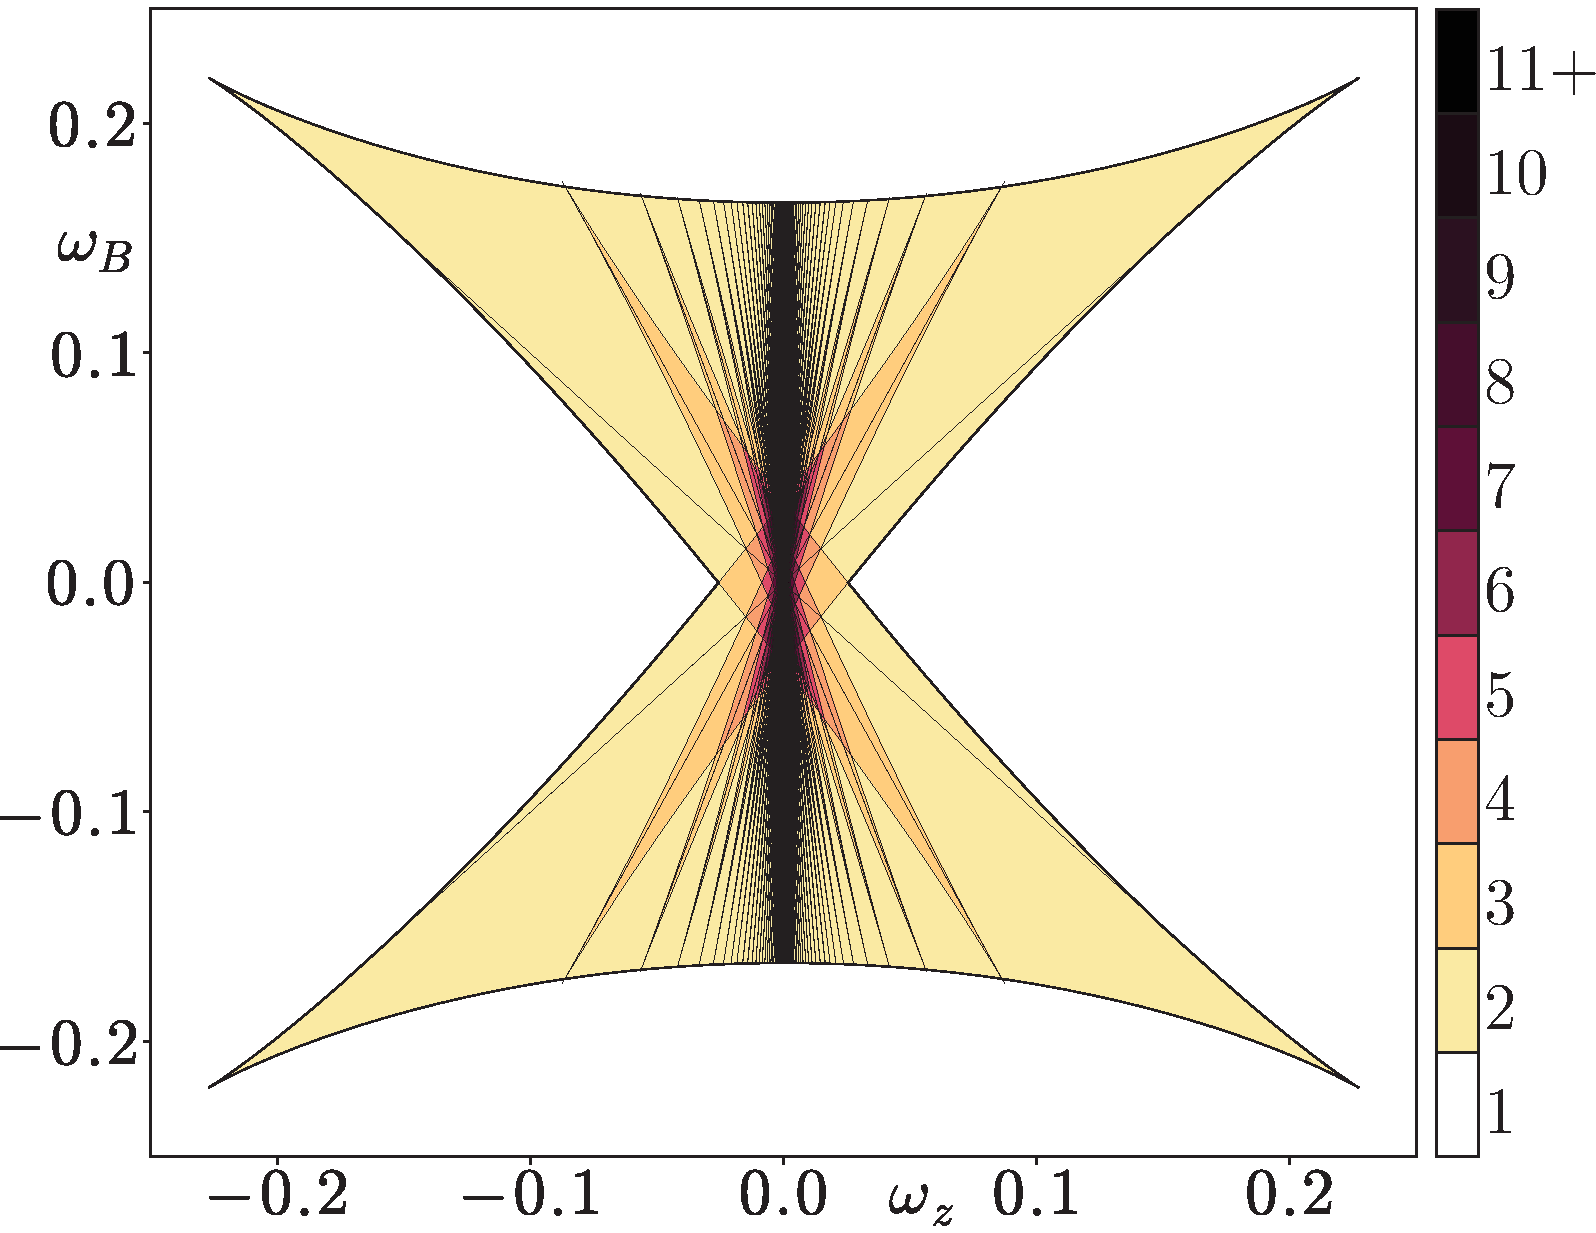
\includegraphics[width=\linewidth]{Images/EGM_components_2D_coloured.pdf}

    \caption{Caption.}
    
    \label{fig:EGM_components}
\end{figure}
%
Figure~\ref{fig:Naumenko_rB003} compare results obtained by both the multiple EC reflection FBG feedback and discretised FBG models for varying grating reflectivity, bandwidth and detuning. 
In order to to obtain valid EGM solutions, for both parameter sets, $N=10 > N_\text{min}=7$ was used. 
Solutions are projected in the frequency-intensity plane where $I = |E|^2$, in contrast to the usual projection in the inversion-frequency plane, causing an inversion of the cavity modes about the frequency axis. 
The photon lifetime $\tau_p=24\,\text{ps}$ was used to convert grating bandwidths in Hz to their nondimensionalised $\wz$ form. 
Clearly, excellent agreement in the mode structure is achieved, in particular for the low feedback rate case. 
Firstly, considering no detuning, low feedback and varying bandwidths as is the case in Figure~\ref{fig:Naumenko_rB003}, 
for a wide bandwidth of the Bragg reflector (in this case, a main lobe width of 40/3 GHz or $2\wz=0.64\pi$ in nondimensionalised form), EGMs lie on a closed curve, resembling a COF ECM structure, as expected. 
The MGM (mode with highest power) is located for near the edge of the left side of the closed curve, indicated by an '$\times$' in the figure. 
As the FBG bandwidth is decreased, the number of EGMs decreases, and the EGM solution curve and MGM narrows as they are confined to within the bandwidth of the main lobe, 
in agreement with results obtained from Sections~\ref{sec:EGM_Lorentzian} and \ref{sec:EGM_discretised} and with results obtained for a single Lorentzian filter \cite{yousefi1999dynamical}. 
Further narrowing the filter bandwidth introduces satellite EGMs, indicated with triangles, due to the side lobes of the FBG reflection spectrum. 
It is noted that this effect does not occur in the single Lorentzian filter for zero detuning. 
At this point, the MGM as nearly at the Bragg frequency, in agreement with physical intuition. 
Increasing the feedback rate considerably, and detuning the FBG from the laser's free-running frequency, as shown in Figure~\ref{fig:Naumenko_rB02}, 
also detune the EGM modes, and split the modes into three disjoint curves, corresponding to the main lobe and two side lobes nearest to the laser's free-running frequency. 
This splitting of solution curves was similarly observed for the single Lorentzian filter \cite{yousefi1999dynamical}, but at most two disjoint curves can be formed \cite{green2006mode}, while in this case already three distinct solution curves are present. 
Significant distortion in the EGM structure along the intensity axis can be seen for the discretised reflection case compared to the Multiple EC reflection model, 
which can be attributed to the lack of a gain suppression factor in this model in this simplified model. 
In any case, excellent agreement in the locations of the EGM components, MGM, and number of EGM solutions demonstrates the ability of the discretised reflections model to capture the solution structure of FBG feedback.
%
\par
%
\subsection{Stability Fluctuations}
\label{subsec:lichaos_skenderas}
%
\begin{figure}[t]
    
    \begin{overpic}[width=\linewidth]{Images/Reflection_zero_overlap.pdf}
        \put(2,86){(a)}
        \put(2,43){(b)}
    \end{overpic}

    \caption{Caption}
    
    \label{fig:zero_overlap}
\end{figure}
%
It is important to note that while the locations of zeros in the discretised model are uniform, is only the case for FBGs which have relatively low reflectivities, see Figure~\ref{fig:uniform_spectra_varykL}. 
For this, re
%

\begin{figure}[t]
    \flushleft
    \begin{overpic}[width=0.845\linewidth]{Images/Li_chaos_heatmap_image.pdf}
        \put(-2,77){(a)}
    \end{overpic}\\
    \vspace{-0.5em}
    \begin{overpic}[width=0.995\linewidth]{Images/discretised_Lichoatic_wBeta_comparison_hopfs.pdf}
        \put(-2,65){(b)}
    \end{overpic}\\
    \vspace{-0.5em}
    \begin{overpic}[width=\linewidth]{Images/discretised_Lichoatic_wBeta_comparison_lyapunovs.pdf}
        \put(-2,70){(c)}
    \end{overpic}

    \caption{Comparison between two parameter dynamical mappings of output intensity for a convolved FBG feedback form of $F(t)$ \cite{li2012distributed,li2015chaotic,li2020stable} (a) 
    and the discretised FBG feedback form of $F(t)$ in the parameter space of feedback strength ($\xi_f$ in (a) and equivalent $\eta$ in (b)) 
    and grating detuning frequency ($\Delta f$). 
    In (a), the laser output intensity is stable (white), period-one oscillatory (red), quasi-periodic pulsating (gray), period-doubled oscillatory (yellow), and chaotic (black). 
    In (b), the laser output is in steady-state (white), period-one oscillatory (red), period-two (yellow), and period 3 to very large period in a gradient from grey to black. 
    In (c) parameter sweeps are performed in all four directions, with Hopf bifurcations of steady state EGMs overlayed.}
    
    \label{fig:Li_chaos}
\end{figure}
%
\par
%
Finally, we compare our model to the most recent work on semiconductor lasers under FBG feedback by \Skenderas \textit{ et al.} \cite{skenderas2021feedback,skenderas2024impact}. 
In contrast to the previous two models, where nondimensionalisations and approximations were required before direct comparisons could be made, the form of the equations analysed mirror the equations presented in this work, 
using parameter values $(\a, P, T, \tau) = (3, 1, 1000, 1000)$, except for the use of a convolution feedback term $F(t)$ of the form \eqref{eq:convolution}. 
The results presented by \Skenderas \textit{ et al.} therefore serve as the most suitable basis for comparisons in the accuracy of the derived discretised model. 
Given the complexity of analysing the LK equations under FBG feedback using a convolution term, the results presented, 
like those previously studied, are obtained solely through analysis of time series obtained through numerical integration. 
The main focus of their analysis is in characterising the interplay between the lasers relaxation oscillations (ROs) and the FBG reflection zeros as a function of feedback rate $\eta$ and grating bandwidth $\wz$ for varying feedback phase $C_p$ and grating detuning $\omega_B$. 
%
\par
%
ROs are the most typical type of oscillation that one would expect in semiconductor lasers. 
They are damped intensity fluctuations that occur when the laser transitions between steady states, typically after a sudden change in injection current, 
and arise from the dynamic interplay between photon density and carrier density in the laser cavity. 
When the carrier population is perturbed, it overshoots the steady-state value, causing oscillations in output power at a characteristic frequency known as the relaxation oscillation frequency $\w_\text{RO}=\sqrt{2P/T}$, 
which form the dominant side lobes either side of the centre frequency in the Fourier spectrum of a semiconductor laser. 
Exciting the ROs of a laser can lead to a more unstable laser, and therefore one would expect that lower amount of feedback would cause the laser to transition from steady output to oscillatory and then more unstable outputs. 
%
\par
%
The strategy employed by the authors to observe this behaviour is by tracking the Hopf bifurcation of the steady state of the laser in the $(L_\text{FBG},\eta)$-plane, 
where the grating length $L_\text{FBG}$ can be used to control the grating bandwidth $\wz$ as discussed in \ref{sec:EGM_discretised}. 
As discussed in \ref{sec:FBG}, varying the grating length also changes the grating reflectivity, therefore, when using this model, grating parameters must be simultaneously varied to solely vary its bandwidth. 
This is not an issue with the discretised reflections model as bandwidth $\wz$ and thus length $L_\text{FBG}$ can be varied independent of reflectivity using \ref{eq:wz_approx}
%
\begin{equation}
    L [\text{m}] \approx \frac{\pi c \tau_p}{\wz \neff} 
\end{equation}
%
where $\tau_p$ is the photon lifetime used to rescale time in this form of the LK equations as discussed in Section~\ref{sec:EGM_discretised}.
%
\par
%
\begin{figure}[!t]
    \flushright
    \begin{overpic}[width=\linewidth]{Images/discretised_Skenderas_wzeta_Cpcomparison_N20.pdf}
        \put(-3,55){(a)}
    \end{overpic}\\
    \hspace{-0.5em}
    \begin{overpic}[width=0.98\linewidth]{Images/discretised_Skenderas_wBeta_image.pdf}
        \put(-3,75){(b)}
    \end{overpic}\\
    \hspace{-0.5em}
    \begin{overpic}[width=0.97\linewidth]{Images/discretised_Skenderas_wBeta_comparison.pdf}
        \put(-3,75){(c)}
    \end{overpic}

    \caption{The evolution of Hopf bifurcation tracking the stability fluctuations as a function of $L_\text{FBG}$ at zero detuning for different values of the feedback offset phase $C_p$ equal to 
    $0$ (blue), $\pi /4$ (yellow), $\pi/2$ (violet), $2\pi/3$ (green), $\pi$ (cyan), $3\pi/2$ (maroon), and $7\pi/4$ (orange). Comparison between two parameter dynamical mappings of output intensity for a convolved FBG feedback form of $F(t)$ \cite{li2012distributed,li2015chaotic,li2020stable} (a) 
    and the discretised FBG feedback form of $F(t)$ in the parameter space of feedback strength ($\xi_f$ in (a) and equivalent $\eta$ in (b)) and grating detuning frequency ($\Delta f$). 
    In (a), the laser output intensity is stable (white), period-one oscillatory (red), quasi-periodic pulsating (gray), period-doubled oscillatory (yellow), and chaotic (black). 
    In (b), the laser output is in steady-state (white), period-one oscillatory (red), period-two (yellow), and period 3 to very large period in a gradient from grey to black. 
    In (c) parameter sweeps are performed in all four directions, with Hopf bifurcations of steady state EGMs overlayed}
    
    \label{fig:Skenderas_wBeta}
\end{figure}
%

